%% ГОСТ 7.32-2017
%% 5.11 Приложения
%%
%% 5.11.1 В приложения рекомендуется включать материалы, дополняющие текст отчета, связанные с выполненной НИР, если они не могут быть включены в основную часть.
%%
%% В приложения могут быть включены:
%% - дополнительные материалы к отчету;
%% - промежуточные математические доказательства и расчёты;
%% - таблицы вспомогательных цифровых данных;
%% - протоколы испытаний;
%% - заключение метрологической экспертизы;
%% - инструкции, методики, описания алгоритмов и программ, разработанных в процессе выполнения НИР;
%% - иллюстрации вспомогательного характера;
%% - копии технического задания на НИР, программы работ или другие исходные документы для выполнения НИР;
%% - протокол рассмотрения результатов выполненной НИР на научно-техническом совете;
%% - акты внедрения результатов НИР или их копии;
%% - копии охранных документов.
%%
%% 5.11.2 Приложения к отчету о НИР, в составе которых предусмотрено проведение патентных исследований, могут быть включены в отчет о патентных исследованиях, оформленный по ГОСТ 15.011, библиографический список публикаций и патентных документов, полученных в результате выполнения НИР, который должен быть оформлен по ГОСТ 7.1, ГОСТ 7.80, ГОСТ 7.82.
%%
%% 5.11.3 Приложения оформляются в соответствии с 6.17.

%% Методические указания к выполнению, оформлению и защите выпускной квалификационной работы бакалавра
%% 2.12 Приложения
%%
%% Приложения состоят из вспомогательного материала, на который в основной части бакалаврской работы имеются ссылки.
%% Приложением оформляют различные схемы, листинг программ, наборы тестов и др.
%%
%% В тексте РПЗ на все приложения должны быть даны ссылки.

\chapter*{ПРИЛОЖЕНИЕ А}\label{toc:attachment-a}
\titleformat{\section}{\bigsize\centering\bfseries}{\thesection}{}{}{}{}
\section*{КОЭФФИЦИЕНТ ОПТИЧЕСКОГО ПОГЛОЩЕНИЯ КСЕНОНА}
\addcontentsline{toc}{chapter}{\parbox[b]{\dimexpr\textwidth-21.855pt}{\vspace{6mm}ПРИЛОЖЕНИЕ А КОЭФФИЦИЕНТ ОПТИЧЕСКОГО ПОГЛОЩЕНИЯ КСЕНОНА}}

\noindent Массив частот Xe p=15

\noindent 0.02000 0.10000 0.19000 0.19400 0.19453 0.19463 0.19500 0.20300 0.20358 0.20368 0.20400 0.21900 0.21963 0.21973 0.22020 0.23700 0.23762 0.23770 0.23820 0.25000 0.27000 0.27058 0.27068 0.27120 0.27300 0.27674 0.27679 0.27681 0.27685 0.27700 0.28500 0.30227 0.30231 0.30233 0.30237 0.30608 0.30612 0.30614 0.30618 0.31000 0.31525 0.31533 0.31537 0.31545 0.31999 0.32003 0.32723 0.32725 0.32737 0.32741 0.32743 0.32747 0.33160 0.33165 0.33167 0.33172 0.33506 0.33510 0.33512 0.33516 0.33587 0.33591 0.33593 0.33597 0.33840 0.33860 0.34010 0.34015 0.34017 0.34021 0.35670 0.35674 0.35676 0.35680 0.35937 0.35941 0.35943 0.35947 0.36222 0.36230 0.36232 0.36240 0.36286 0.36290 0.36292 0.36296 0.36440 0.36444 0.36446 0.36450 0.36552 0.36556 0.36558 0.36562 0.38030 0.38034 0.38036 0.38040 0.39252 0.39256 0.39258 0.39262 0.40540 0.42130 0.44120 0.48390 0.50000 0.52630 0.55550 0.58820 0.62406 0.63366 0.63372 0.63830 0.64221 0.64225 0.64873 0.64878 0.66650 0.66654 0.69770 0.83330 1.03448 1.20000 1.40000 1.60000 1.94100 2.00100 2.02100 2.02500 2.03200 2.03500 2.03900 2.04000 2.04040 2.04050 2.04120 2.04152 2.04220 2.04240 2.04280 2.04340 2.04700 2.05000 2.05500 2.06100 2.08100 2.14100 2.21555 2.26550 2.29500 2.30000 2.31000 2.31355 2.31470 2.31525 2.31535 2.31540 2.31545 2.31565 2.31570 2.31575 2.31585 2.31630 2.31755 2.32000 2.33000 2.33500 2.36550 2.38460 2.38960 2.39660 2.39860 2.39930 2.39950 2.39970 2.40000 2.40060 2.40260 2.40960 2.41460 2.50670 2.51000 2.51578 2.51648 2.51668 2.51673 2.51683 2.51688 2.51708 2.51778 2.52000 2.52670 3.00000

\noindent Массив коэффициента поглощения Xe p=15 T=3000

\noindent .564e-2 .614e‑2 .643e‑2 .645e‑2 .646e‑2 .645e‑2 .648e‑2 .652e‑2 .644e‑2 .652e‑2 .657e‑2 .661e‑2 .662e‑2 .663e‑2 .668e‑2 .675e‑2 .675e‑2 .675e‑2 .679e‑2 .691e‑2 .699e‑2 .700e‑2 .698e‑2 .700e‑2 .702e‑2 .713e‑2 .706e‑2 .700e‑2 .704e‑2 .707e‑2 .717e‑2 .706e‑2 .723e‑2 .723e‑2 .725e‑2 .731e‑2 .688e‑2 .731e‑2 .728e‑2 .732e‑2 .738e‑2 .730e‑2 .734e‑2 .736e‑2 .742e‑2 .741e‑2 .749e‑2 .745e‑2 .748e‑2 .733e‑2 .748e‑2 .745e‑2 .759e‑2 .745e‑2 .739e‑2 .749e‑2 .753e‑2 .750e‑2 .749e‑2 .751e‑2 .755e‑2 .754e‑2 .747e‑2 .752e‑2 .749e‑2 .754e‑2 .754e‑2 .760e‑2 .733e‑2 .761e‑2 .761e‑2 .780e‑2 .770e‑2 .770e‑2 .772e‑2 .782e‑2 .764e‑2 .772e‑2 .772e‑2 .750e‑2 .775e‑2 .774e‑2 .775e‑2 .784e‑2 .767e‑2 .775e‑2 .757e‑2 .785e‑2 .777e‑2 .776e‑2 .771e‑2 .782e‑2 .781e‑2 .783e‑2 .794e‑2 .795e‑2 .785e‑2 .795e‑2 .797e‑2 .804e‑2 .802e‑2 .807e‑2 .820e‑2 .838e‑2 .870e‑2 .901e‑2 .925e‑2 .958e‑2 .996e‑2 .104e‑1 .107e‑1 .109e‑1 .108e‑1 .109e‑1 .110e‑1 .110e‑1 .111e‑1 .112e‑1 .113e‑1 .115e‑1 .130e‑1 .186e‑1 .280e1 .365e1 .661e1 .363e+0 .365e+1 .177e+2 .435e+2 .946e+2 .243e+3 .963e+3 .447e+4 .109e+5 .170e+5 .769e+5 .417e+6 .775e+5 .160e+5 .945e+4 .487e+4 .125e+4 .297e+3 .123e+3 .541e+2 .187e+2 .389e+1 .137e+1 .222e+1 .915e+1 .287e+2 .106e+3 .819e+3 .530e+4 .331e+5 .120e+6 .198e+6 .291e+6 .469e+6 .279e+6 .191e+6 .116e+6 .366e+5 .594e+4 .102e+4 .141e+3 .327e+2 .985e+1 .425e+1 .694e+1 .267e+2 .248e+3 .234e+4 .195e+5 .210e+6 .213e+5 .199e+4 .259e+3 .266e+2 .615e+1 .121e+1 .308e+1 .299e+2 .915e+3 .305e+5 .165e+6 .299e+5 .699e+4 .250e+4 .431e+3 .507e+2 .579e+1 .141e+0

\noindent Массив коэффициента поглощения Xe p=15 T=4000

\noindent .320e‑2 .348e‑2 .365e‑2 .366e‑2 .366e‑2 .367e‑2 .368e‑2 .370e‑2 .368e‑2 .370e‑2 .373e‑2 .375e‑2 .377e‑2 .376e‑2 .379e‑2 .383e‑2 .384e‑2 .383e‑2 .386e‑2 .392e‑2 .397e‑2 .398e‑2 .397e‑2 .398e‑2 .399e‑2 .405e‑2 .394e‑2 .403e‑2 .399e‑2 .401e‑2 .407e‑2 .406e‑2 .418e‑2 .415e‑2 .412e‑2 .421e‑2 .433e‑2 .423e‑2 .413e‑2 .415e‑2 .419e‑2 .416e‑2 .418e‑2 .418e‑2 .418e‑2 .421e‑2 .425e‑2 .425e‑2 .428e‑2 .423e‑2 .427e‑2 .423e‑2 .432e‑2 .432e‑2 .420e‑2 .425e‑2 .425e‑2 .428e‑2 .429e‑2 .426e‑2 .426e‑2 .427e‑2 .425e‑2 .427e‑2 .426e‑2 .428e‑2 .462e‑2 .544e‑2 .450e‑2 .432e‑2 .436e‑2 .448e‑2 .438e‑2 .437e‑2 .440e‑2 .442e‑2 .437e‑2 .438e‑2 .441e‑2 .422e‑2 .441e‑2 .440e‑2 .442e‑2 .440e‑2 .438e‑2 .440e‑2 .456e‑2 .506e‑2 .458e‑2 .441e‑2 .443e‑2 .446e‑2 .439e‑2 .444e‑2 .451e‑2 .450e‑2 .447e‑2 .451e‑2 .453e‑2 .458e‑2 .453e‑2 .458e‑2 .466e‑2 .476e‑2 .494e‑2 .512e‑2 .525e‑2 .544e‑2 .566e‑2 .591e‑2 .609e‑2 .614e‑2 .615e‑2 .619e‑2 .622e‑2 .623e‑2 .635e‑2 .634e‑2 .638e‑2 .656e‑2 .740e‑2 .106e‑1 .159e‑1 .207e‑1 .375e‑1 .206e+0 .207e+1 .100e+2 .247e+2 .536e+2 .138e+3 .546e+3 .254e+4 .622e+4 .977e+4 .490e+5 .369e+6 .493e+5 .919e+4 .540e+4 .277e+4 .710e+3 .168e+3 .696e+2 .307e+2 .106e+2 .221e+1 .779e+0 .126e+1 .521e+1 .164e+2 .601e+2 .467e+3 .303e+4 .195e+5 .754e+5 .133e+6 .214e+6 .423e+6 .203e+6 .128e+6 .729e+5 .216e+5 .340e+4 .580e+3 .806e+2 .186e+2 .561e+1 .244e+1 .400e+1 .155e+2 .144e+3 .136e+4 .116e+5 .168e+6 .129e+5 .116e+4 .150e+3 .154e+2 .356e+1 .700e+0 .183e+1 .178e+2 .548e+3 .214e+5 .141e+6 .194e+5 .423e+4 .150e+4 .258e+3 .303e+2 .345e+1 .815e‑1

\chapter*{ПРИЛОЖЕНИЕ Б}\label{toc:attachment-b}
\titleformat{\section}{\bigsize\centering\bfseries}{\thesection}{}{}{}{}
\section*{ПРЕЗЕНТАЦИЯ}
\addcontentsline{toc}{chapter}{ПРИЛОЖЕНИЕ Б ПРЕЗЕНТАЦИЯ}


\includegraphics[angle=90,origin=c, height=180mm]{inc/img/presentation-1}

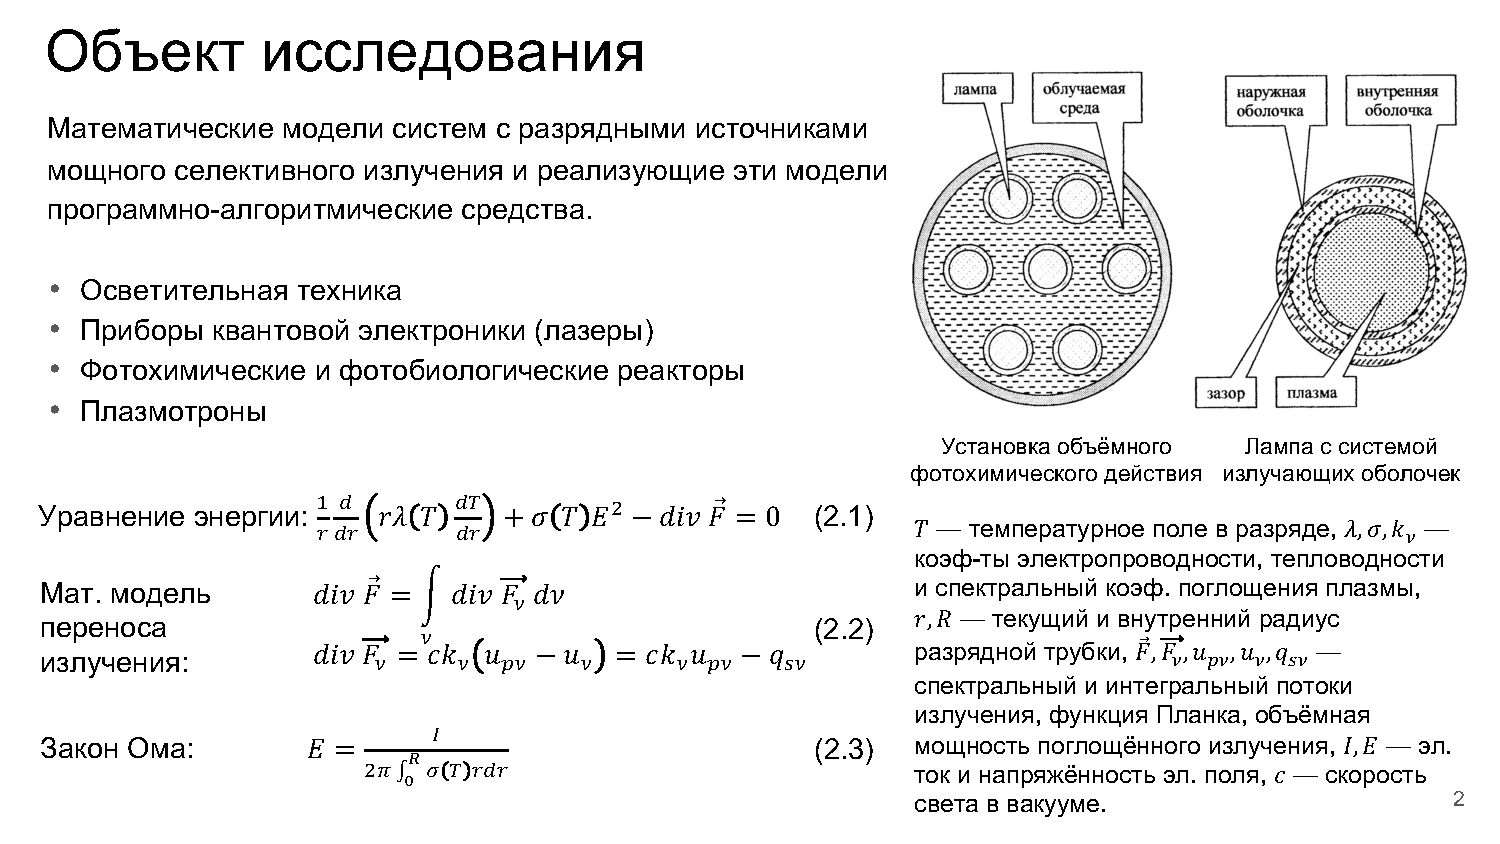
\includegraphics[angle=90,origin=c]{inc/img/presentation-2}

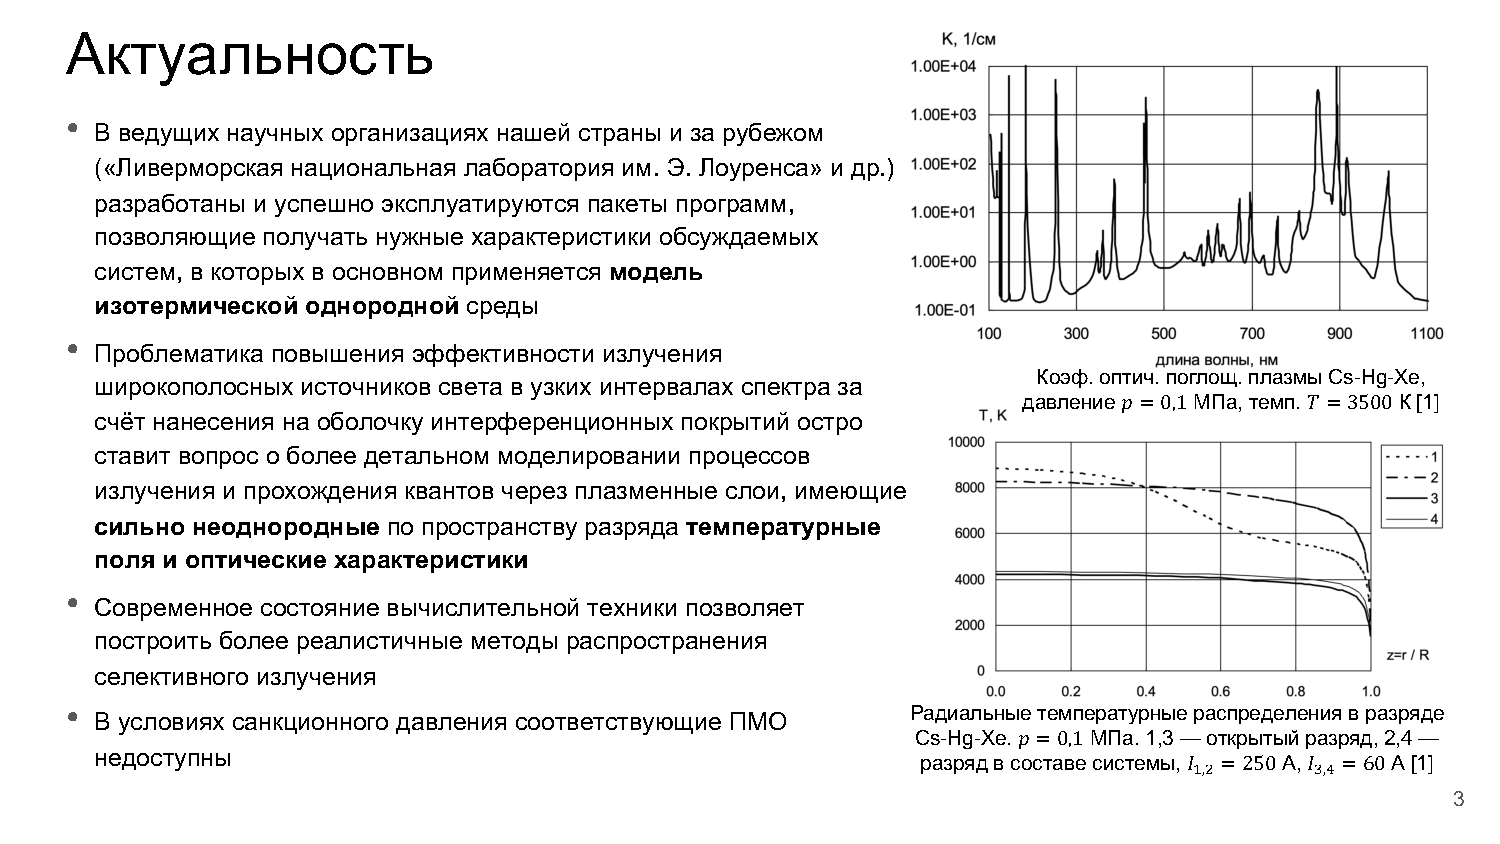
\includegraphics[angle=90,origin=c]{inc/img/presentation-3}

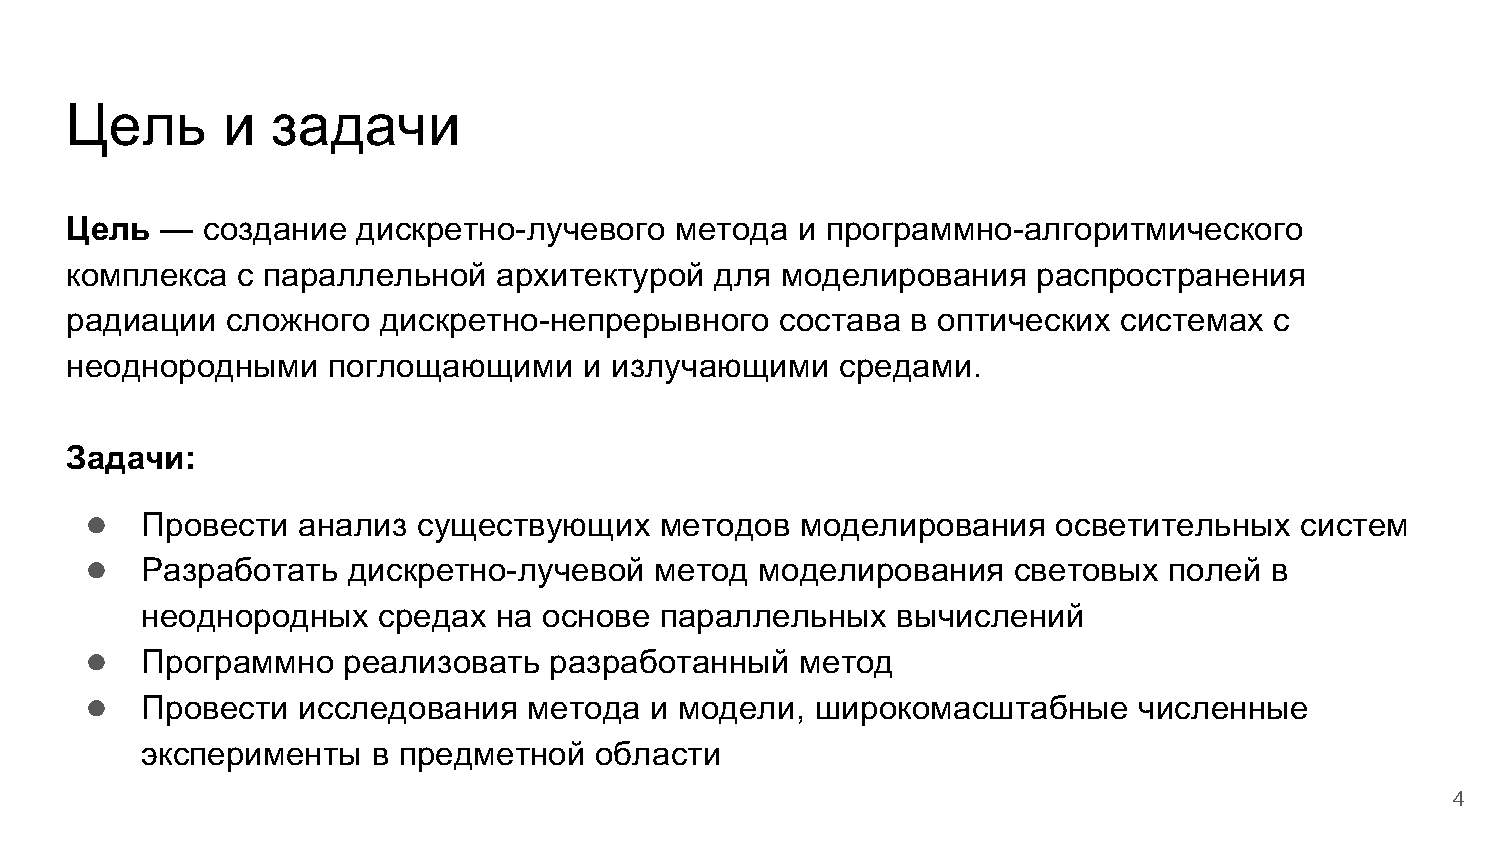
\includegraphics[angle=90,origin=c]{inc/img/presentation-4}

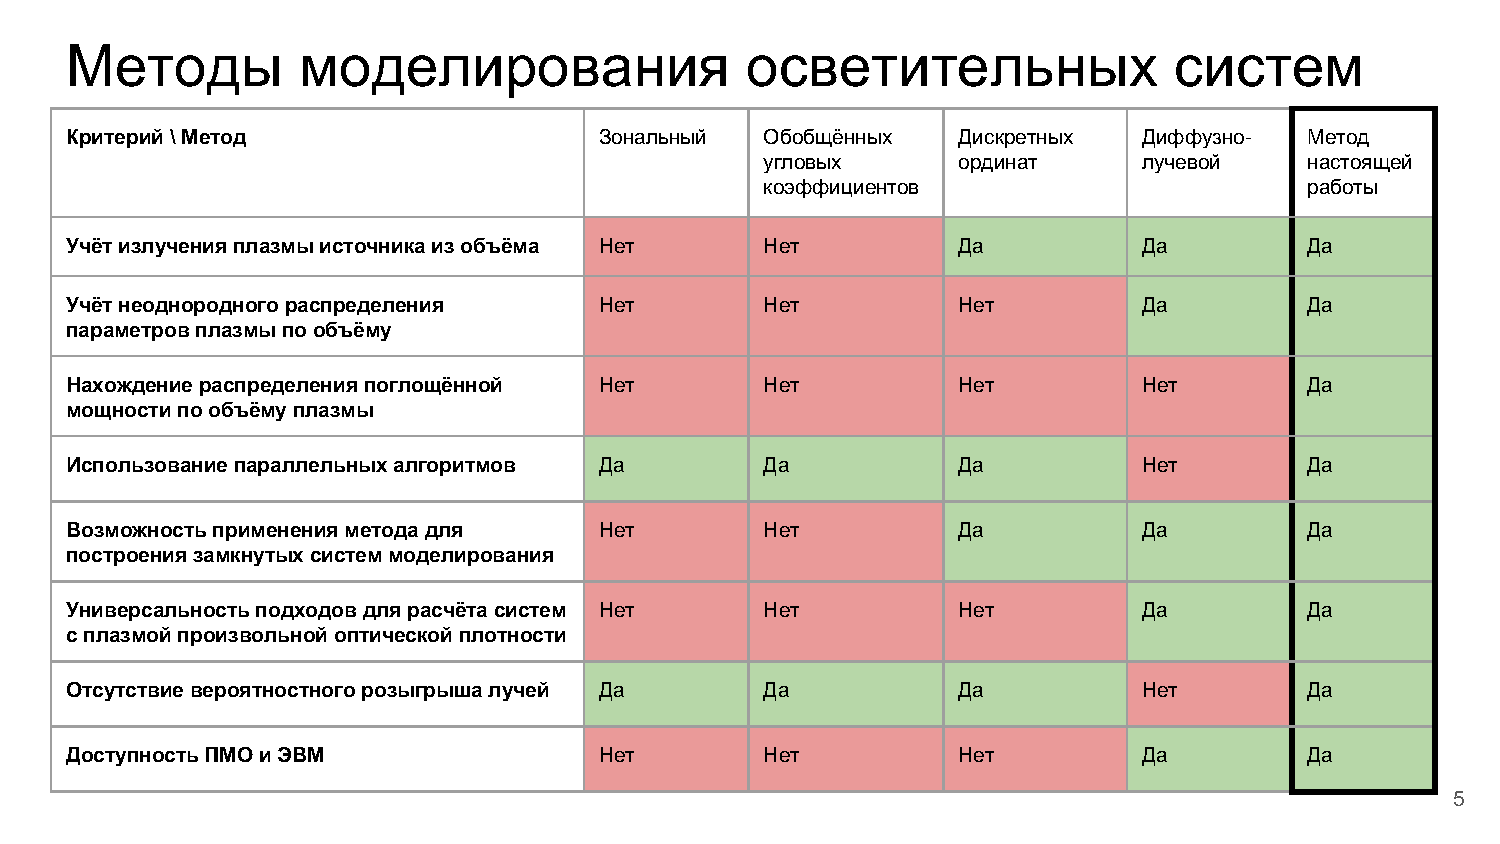
\includegraphics[angle=90,origin=c]{inc/img/presentation-5}

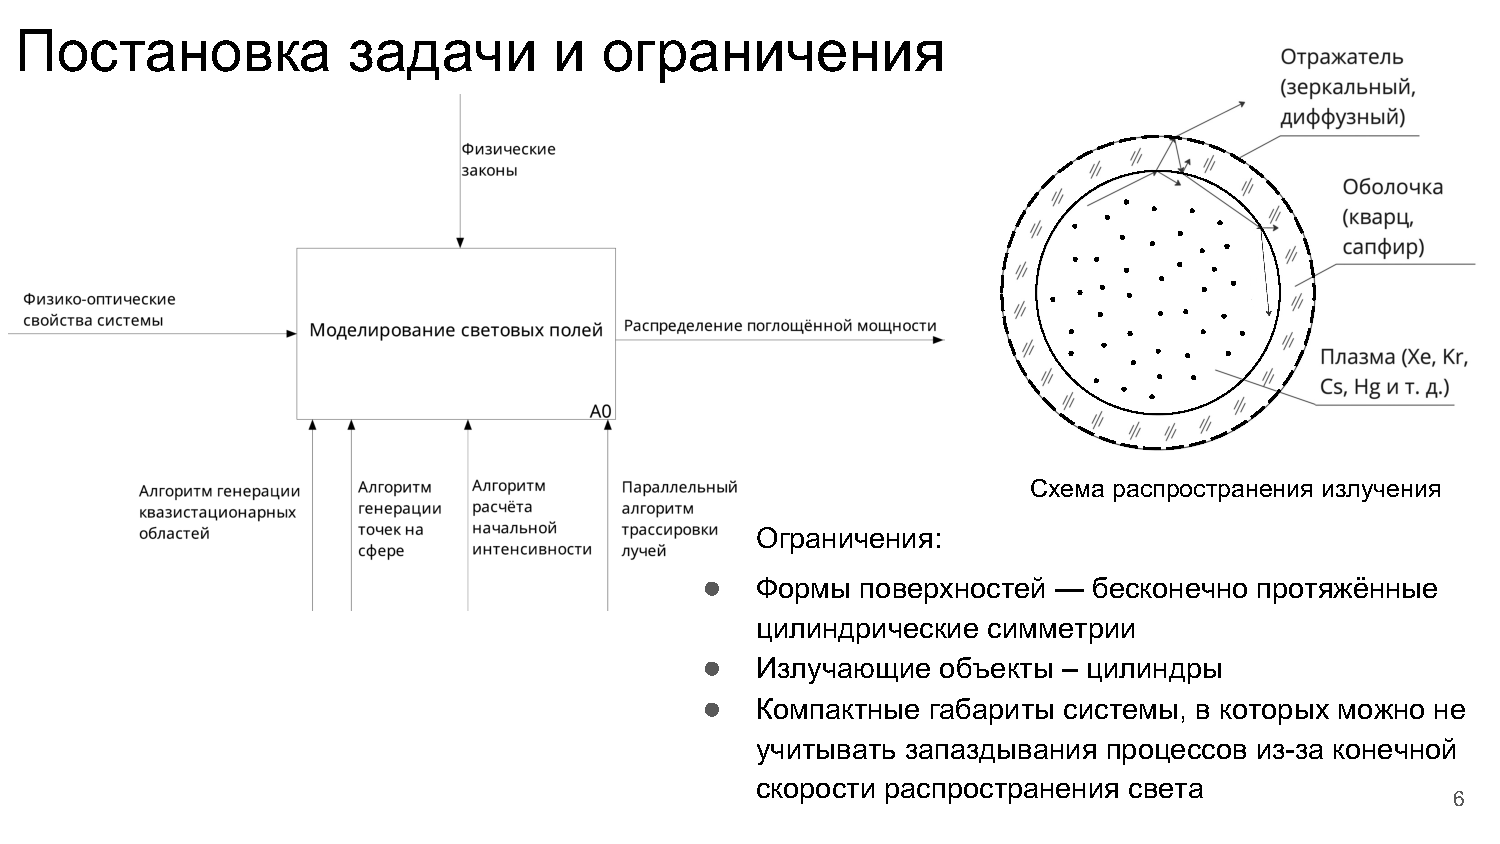
\includegraphics[angle=90,origin=c]{inc/img/presentation-6}

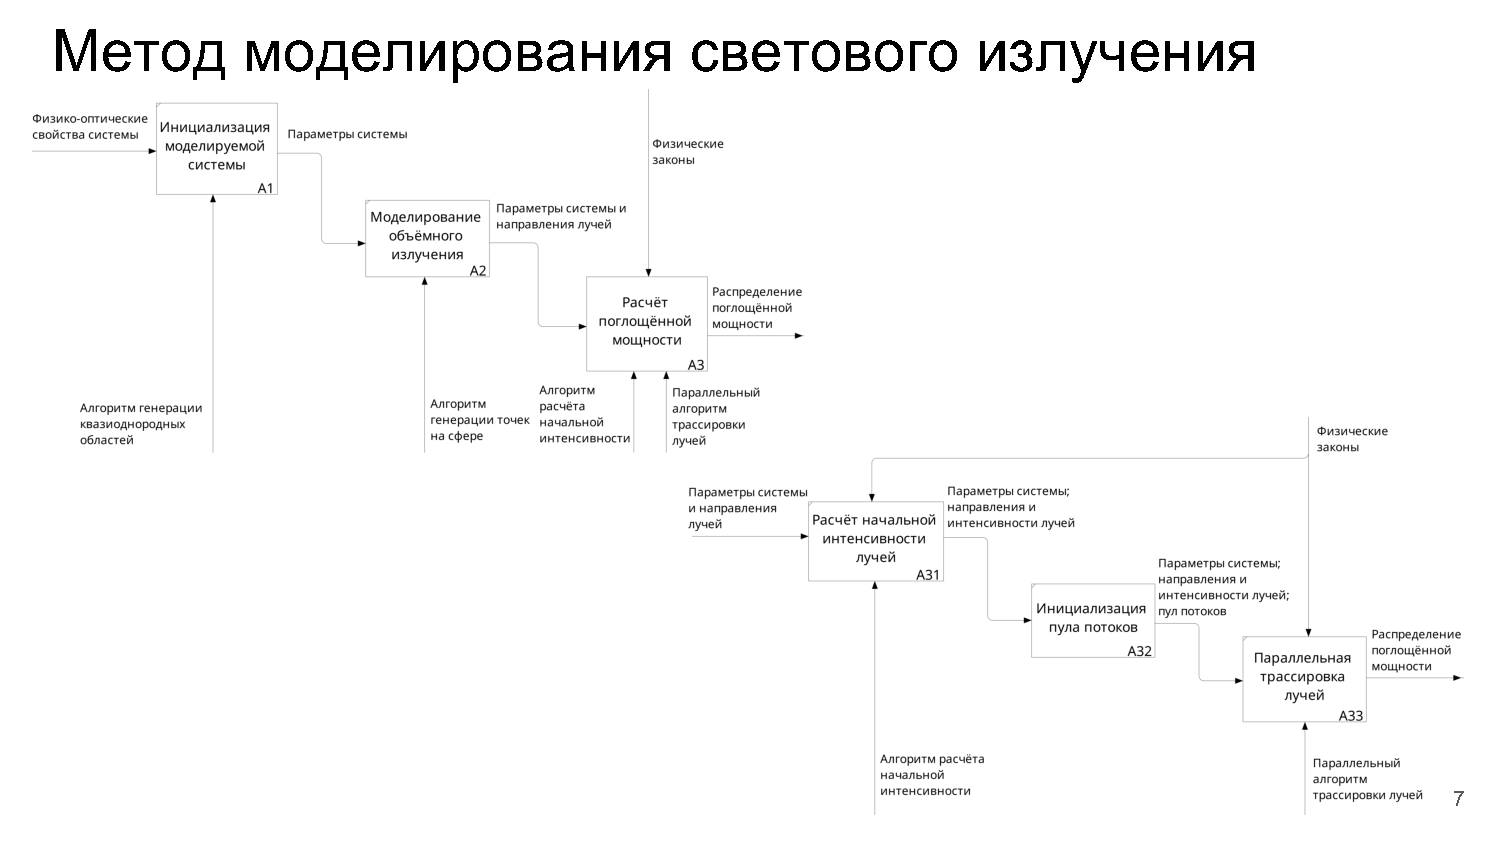
\includegraphics[angle=90,origin=c]{inc/img/presentation-7}

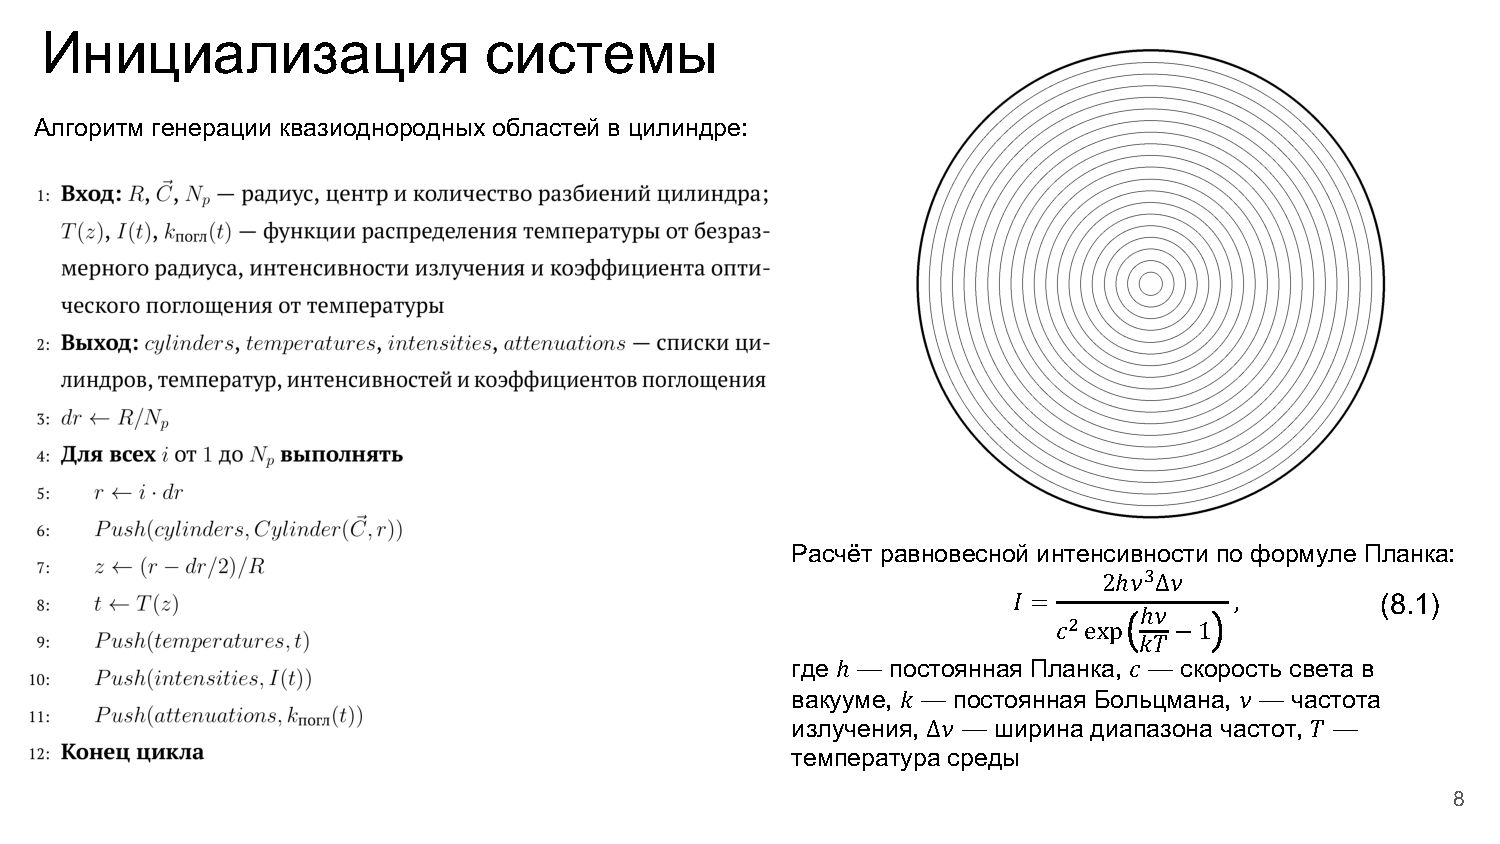
\includegraphics[angle=90,origin=c]{inc/img/presentation-8}

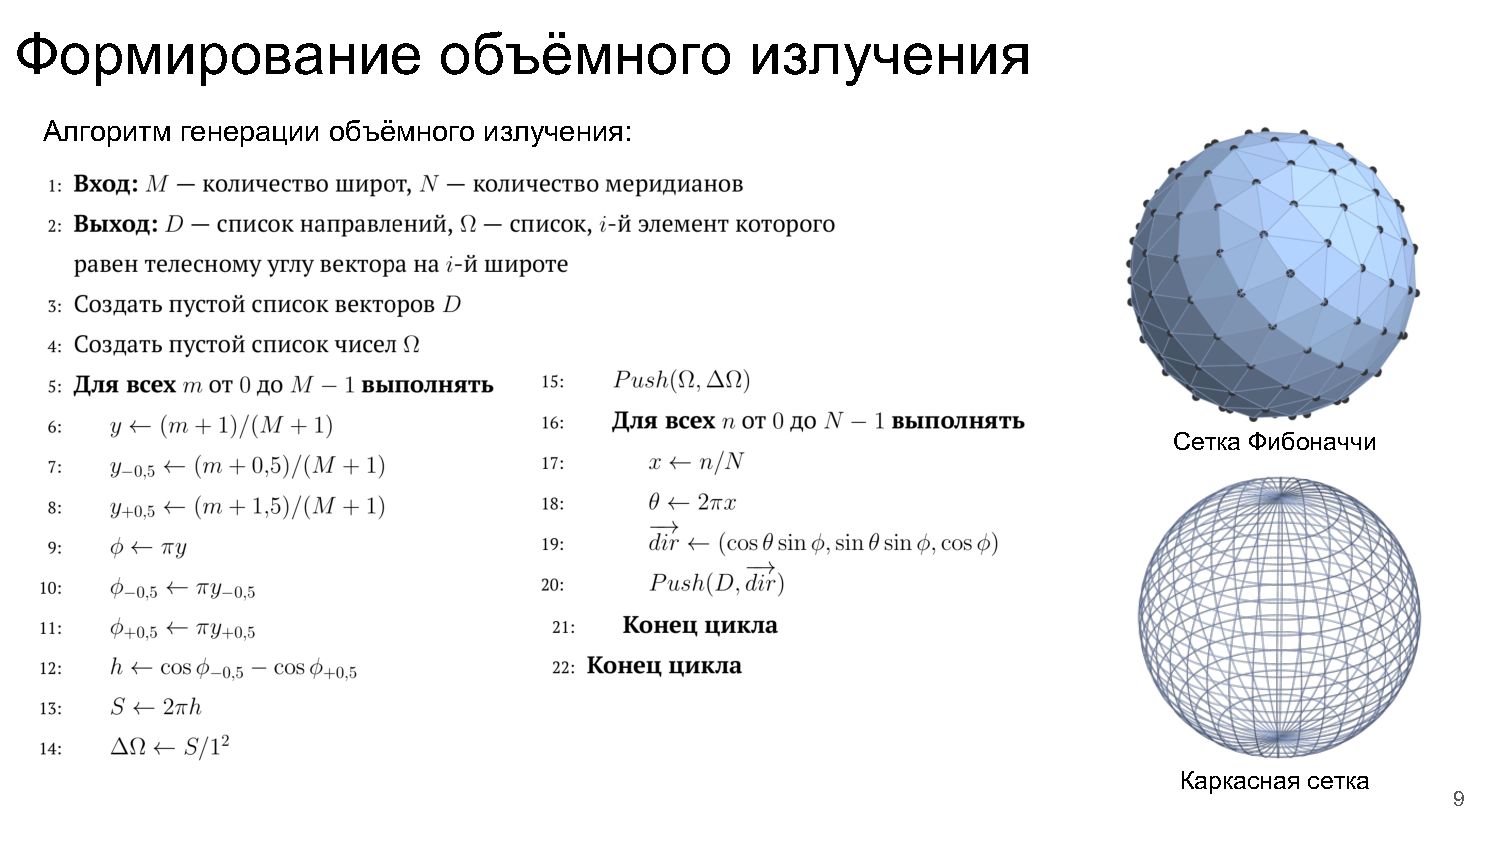
\includegraphics[angle=90,origin=c]{inc/img/presentation-9}

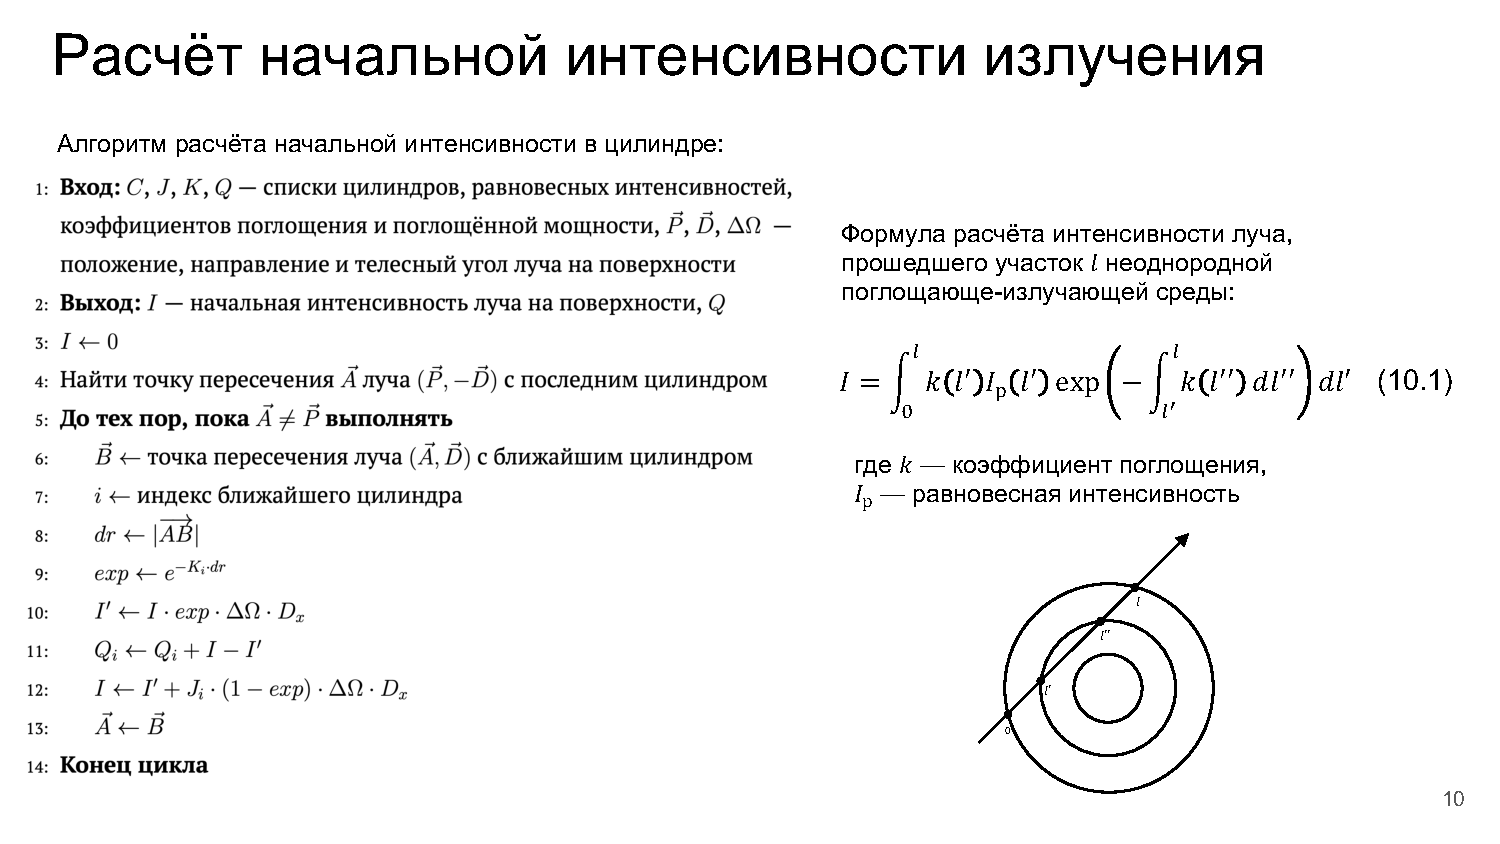
\includegraphics[angle=90,origin=c]{inc/img/presentation-10}

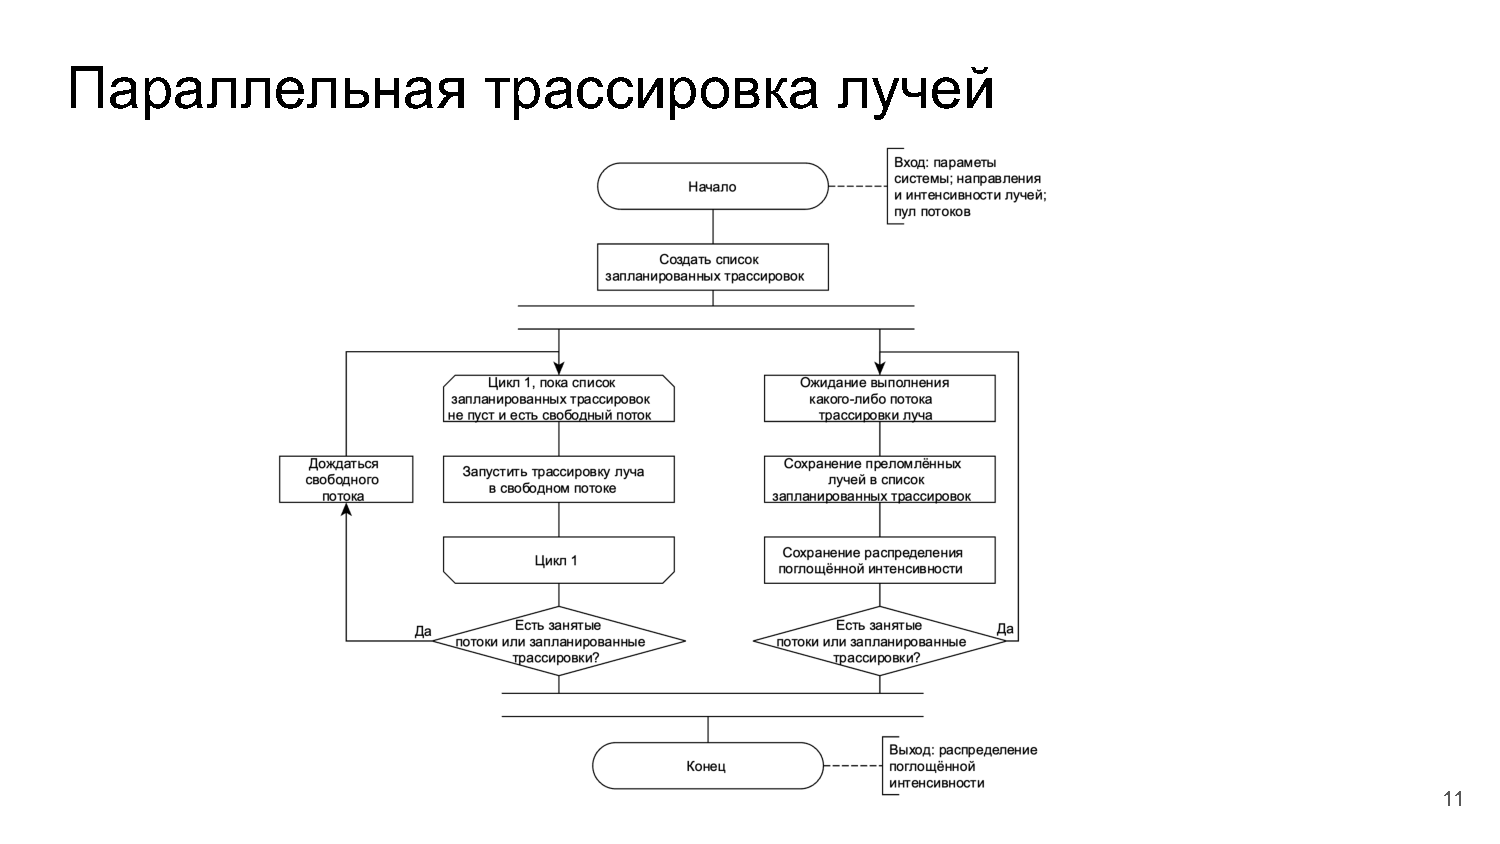
\includegraphics[angle=90,origin=c]{inc/img/presentation-11}

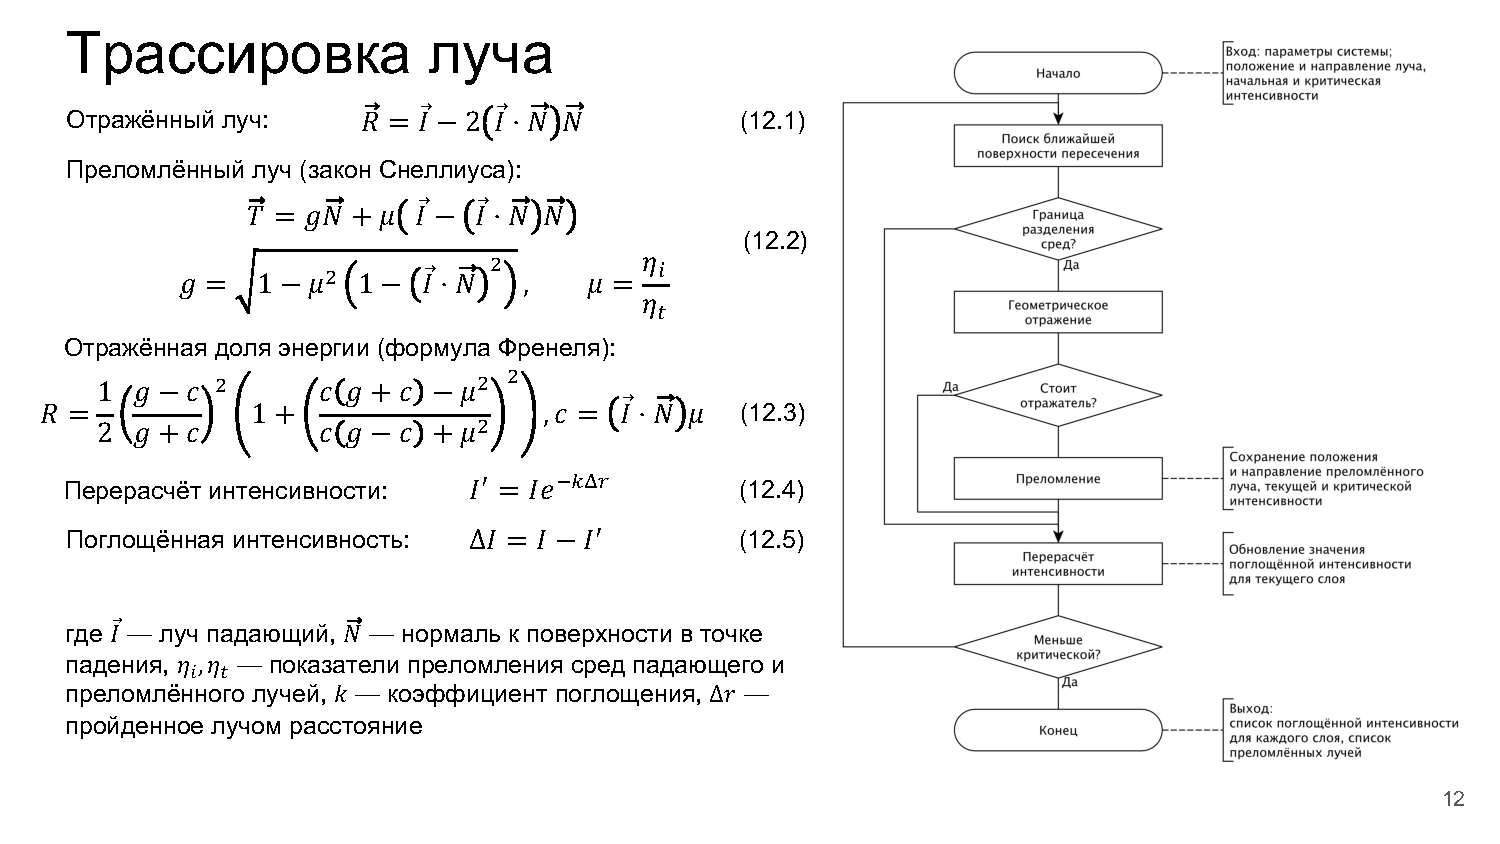
\includegraphics[angle=90,origin=c]{inc/img/presentation-12}

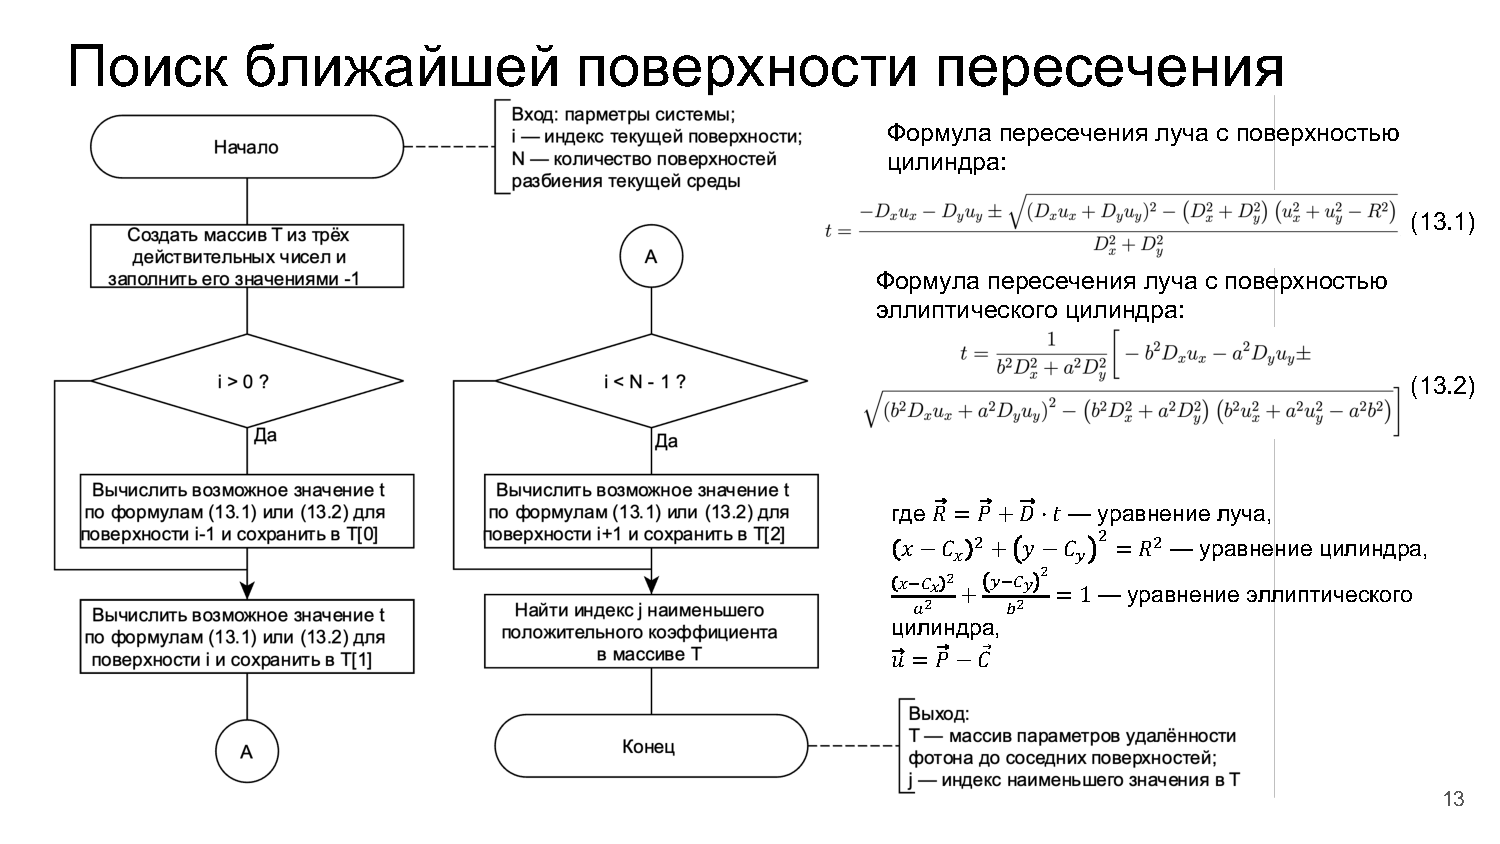
\includegraphics[angle=90,origin=c]{inc/img/presentation-13}

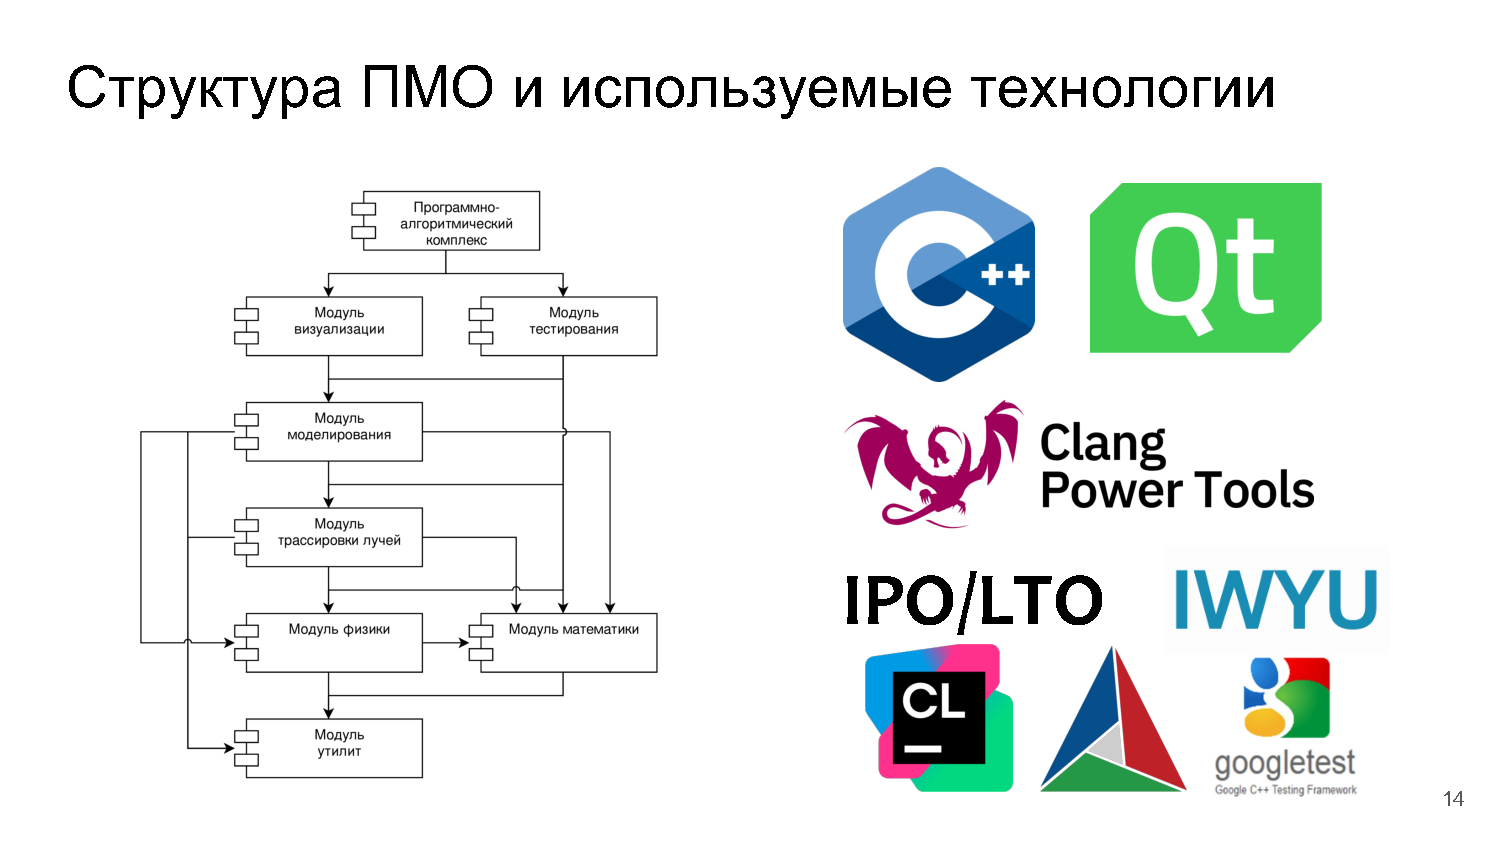
\includegraphics[angle=90,origin=c]{inc/img/presentation-14}

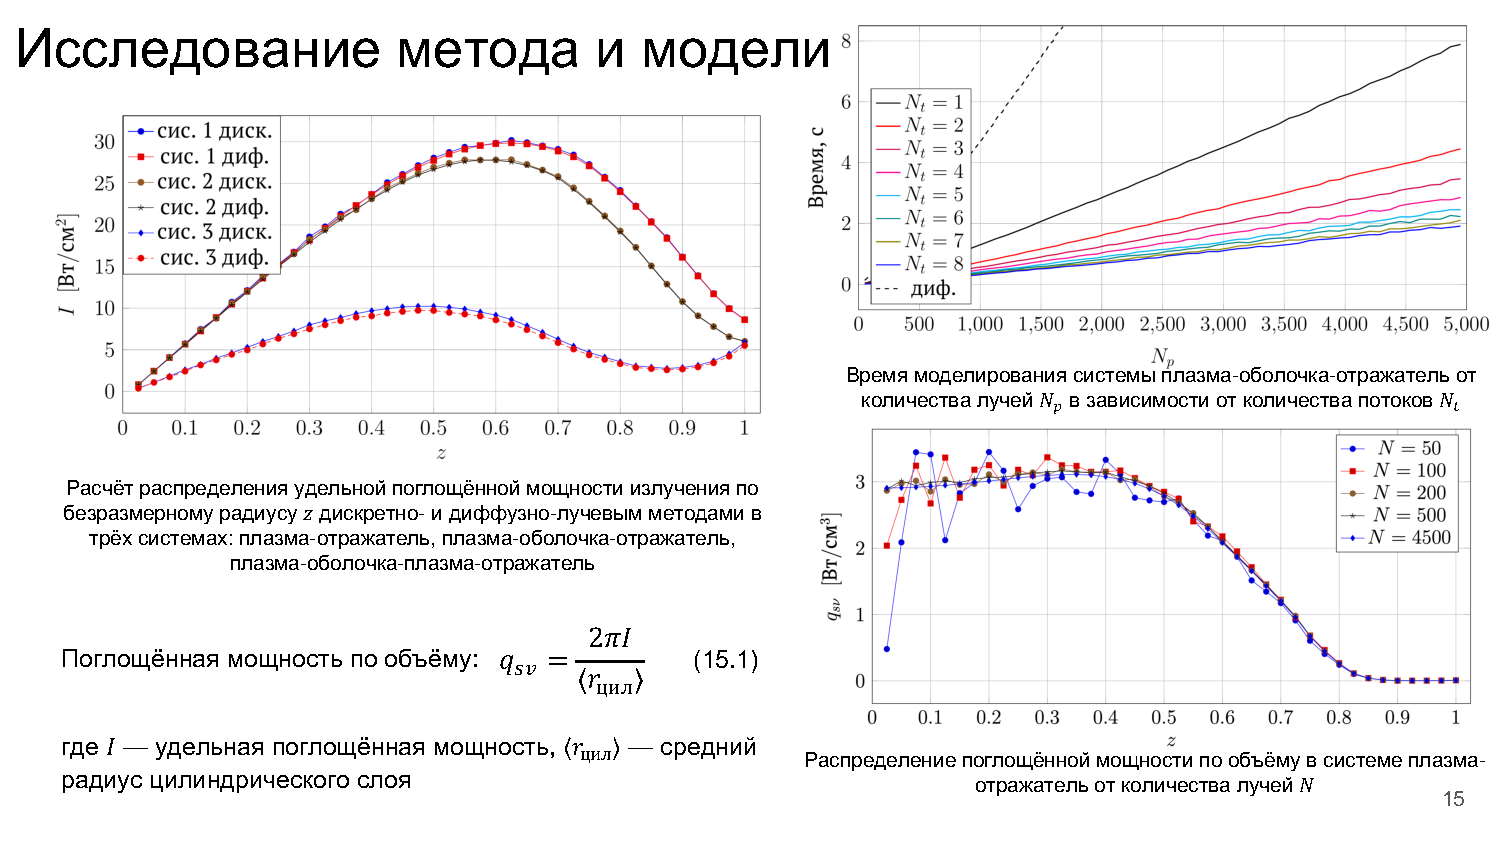
\includegraphics[angle=90,origin=c]{inc/img/presentation-15}

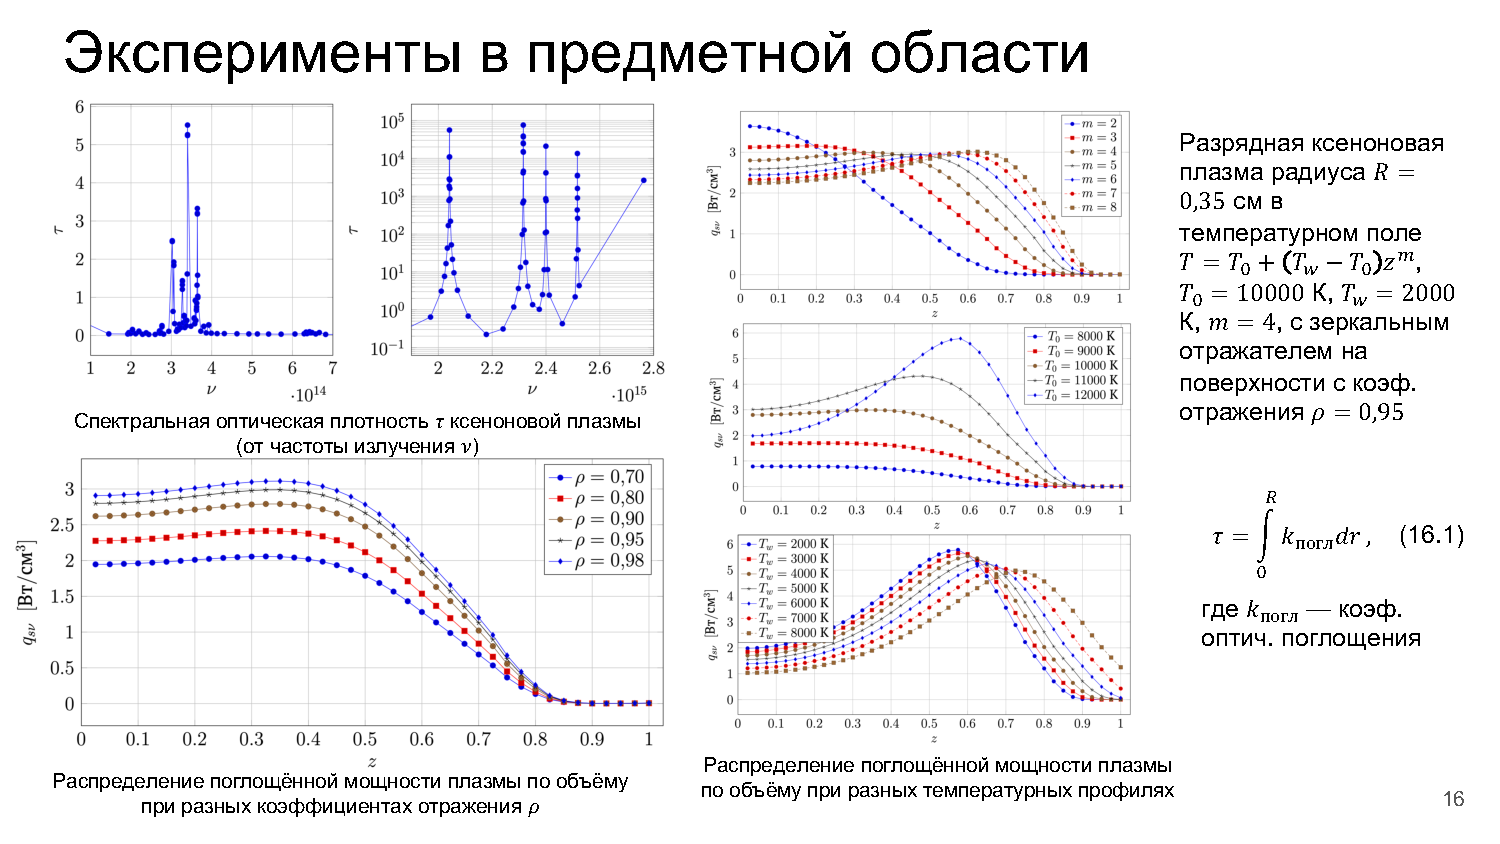
\includegraphics[angle=90,origin=c]{inc/img/presentation-16}

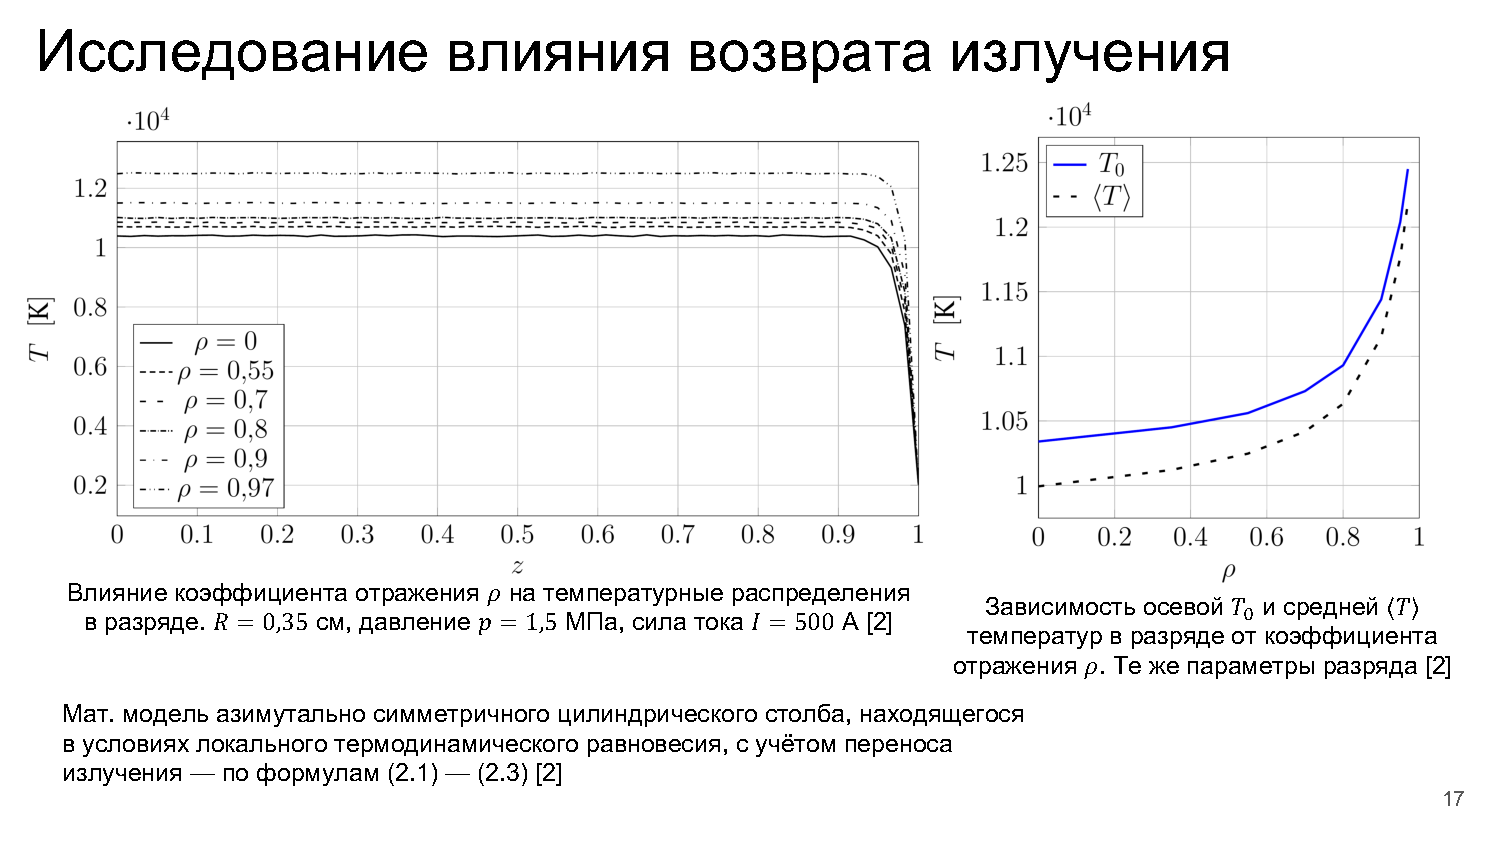
\includegraphics[angle=90,origin=c]{inc/img/presentation-17}

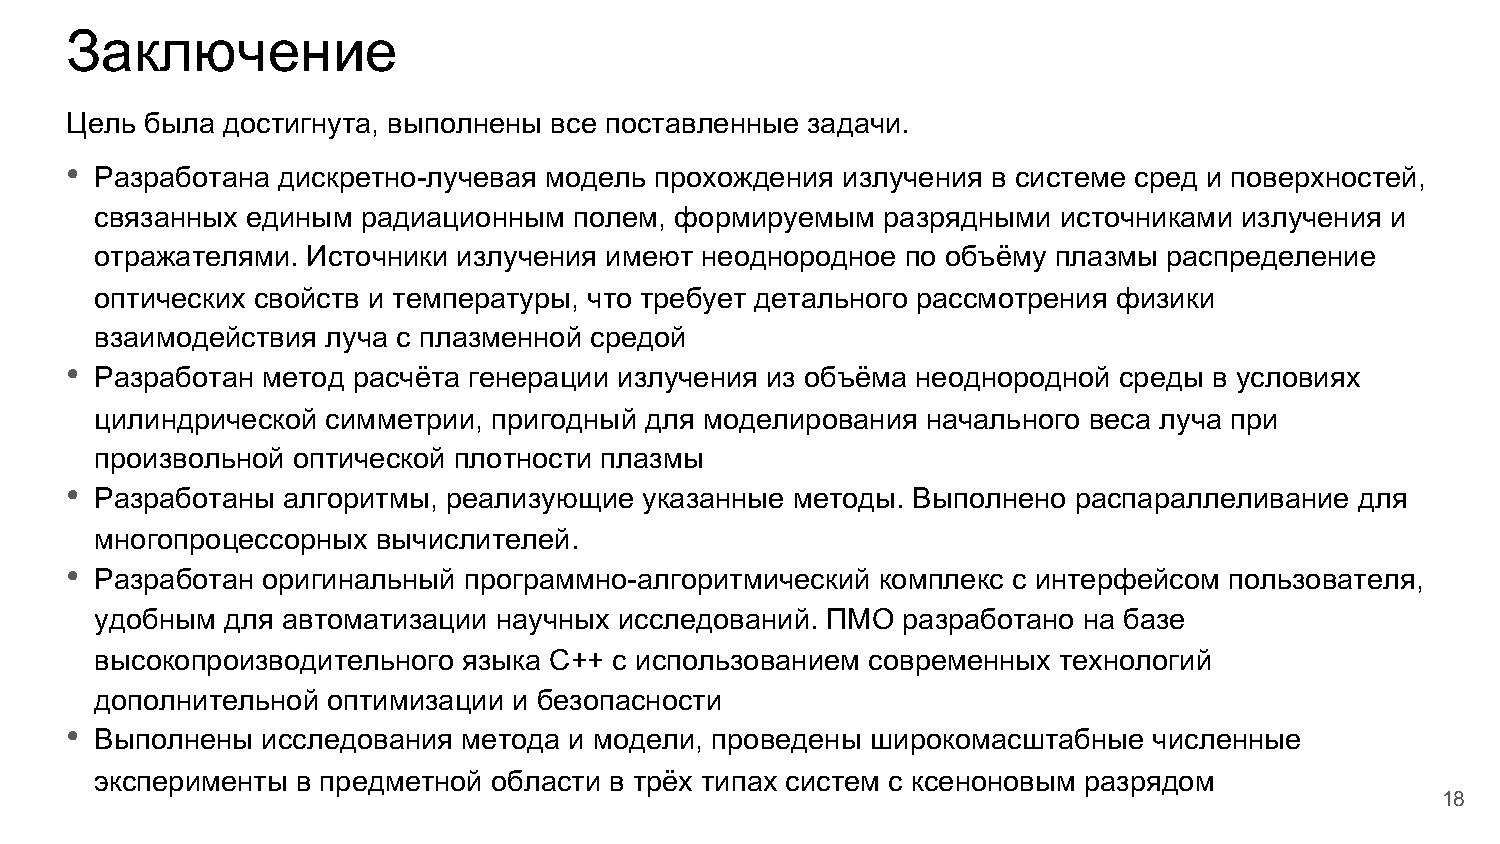
\includegraphics[angle=90,origin=c]{inc/img/presentation-18}

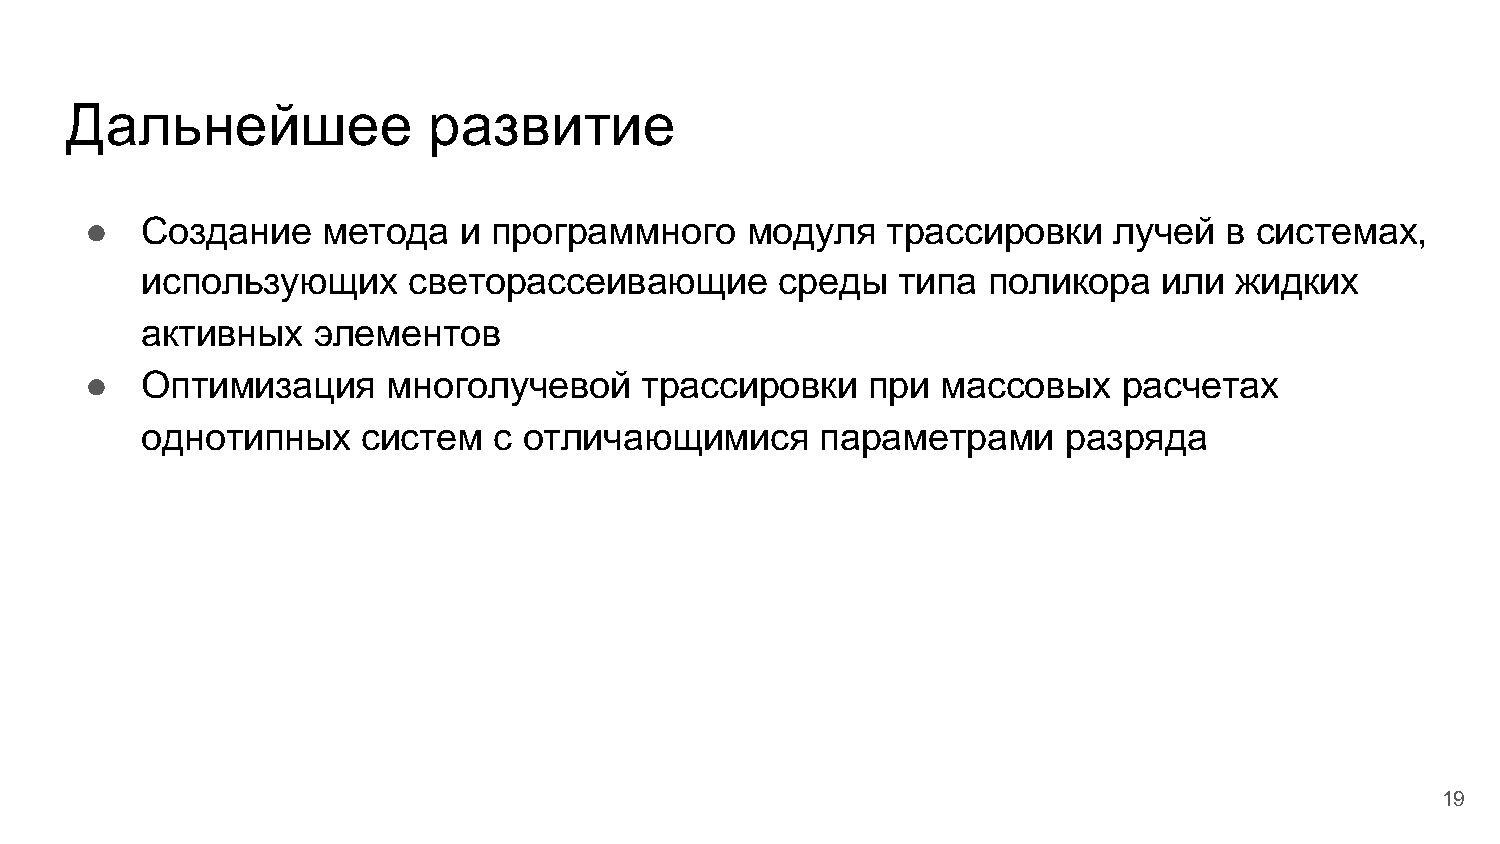
\includegraphics[angle=90,origin=c]{inc/img/presentation-19}

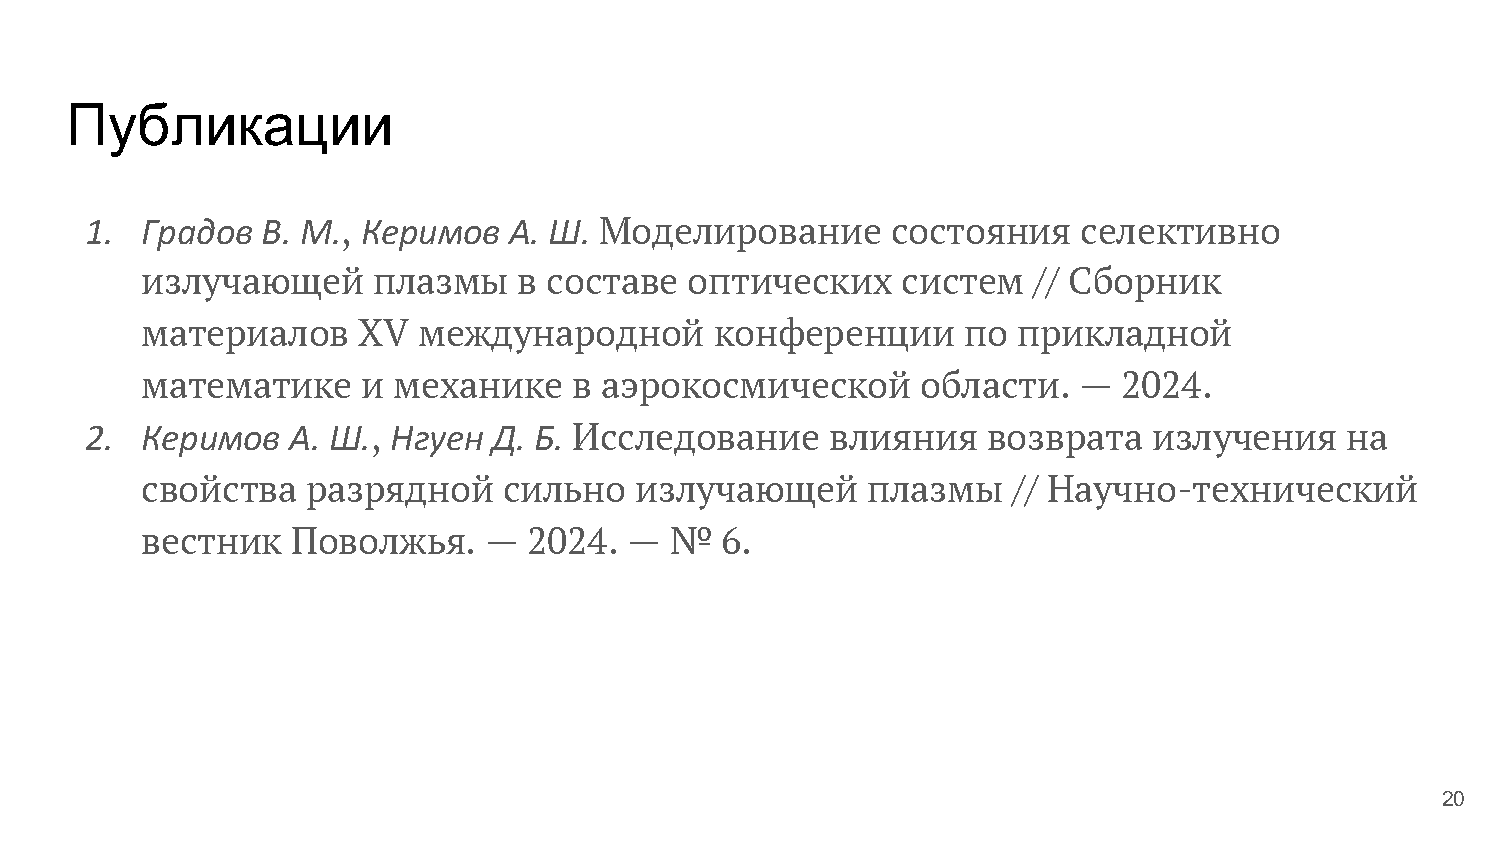
\includegraphics[angle=90,origin=c]{inc/img/presentation-20}
